\chapter{Funcionalidades del producto}

Se presentan las funcionalidades del producto de software Cine+ a través de diagramas Use Case de UML, máquinas de estados UML y otros.

\section{Funcionalidades relacionadas con el gerente}

Como se observa en la Fig \ref{fig:gerente}, existe un actor denominado Gerente el cual se relaciona con varios casos de uso, los cuales representan las funcionalidades del producto relacionadas con el gerente.

\begin{figure}[h!]
    \centering
    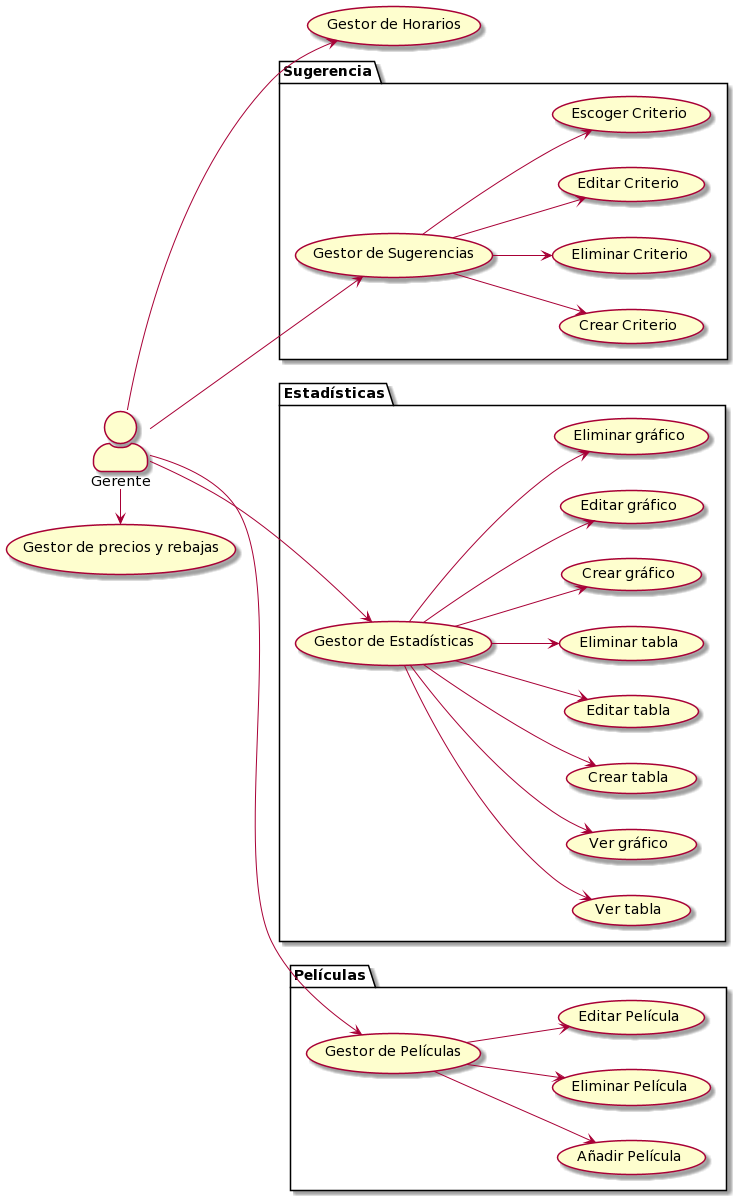
\includegraphics[width=7cm]{./chapters/img/gerente.png}

    \label{fig:gerente}
    \caption{Use Case de las funcionalidades del gerente}
\end{figure}

A continuación se explican cada una de las funcionalidades:

\begin{enumerate}
    \item[$\bullet$] \textbf{Gestor de Películas:} éste pertenece al paquete de casos de uso Películas. Una vez el gerente acceda al gestor, podrá añadir o eliminar películas a proyectar en el cine, así como modificar sus campos mencionados en el Capítulo \ref{ch:model}. Así como habilitar la proyección en un horario en específico del cine.
    \item[$\bullet$] \textbf{Gestor de Horarios:} a través de este caso de uso, se pueden añadir, modificar, o eliminar horarios para las proyecciones.
    \item[$\bullet$] \textbf{Gestor de Estadísticas:} éste pertence al paquete Estadísticas. Una vez el gerente acceda al gestor, podrá añadir tablas a las estadísticas (que no serán más que consultas a las tablas de la base de datos), eliminarlas, editarlas, o visualizarlas. Además puede añadir, eliminar, editar o visualizar los gráfico utilizando el script \href{https://www.chartjs.org}{Charts.js}.
    \item[$\bullet$] \textbf{Gestor de Sugerencias:} donde el gerente puede seleccionar un criterio para seleccionar las películas, así como crear un nuevo criterio, eliminarlo, o modificarlo.
    \item[$\bullet$] \textbf{Gestor de Precios y Rebajas:} el gerente puede definir los porcientos de rebajas y las razones de rebajas, así como eliminar o editar los mismos. Así como definir los precios de las entradas. 
\end{enumerate}

\section{Funcionalidades relacionadas con el cliente y el taquillero}

Como se observa en la Fig \ref{fig:cltq}, existe un actor denominado Cliente y otro Taquillero que representan estos usuarios del sistema, los cuales se relacionan con distintos casos de uso.

\begin{figure}[h!]
    \centering
    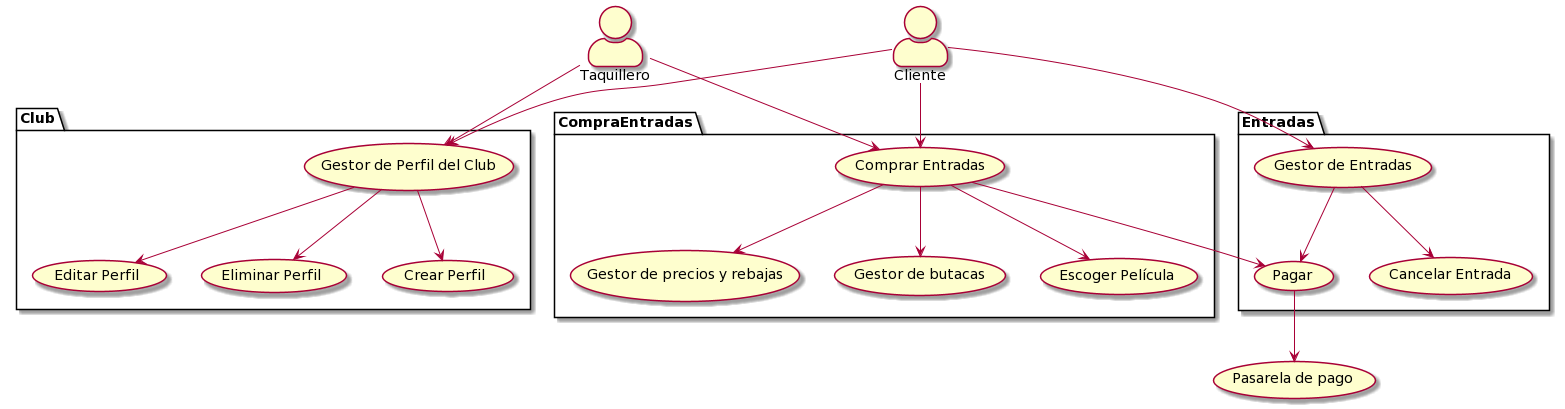
\includegraphics[width=\linewidth]{./chapters/img/cliente-taquillero.png}
    
    \label{fig:cltq}
    \caption{Use Case de las funcionalidades del cliente y el taquillero}
\end{figure}

\subsection{Relacionadas con el cliente}

A continuación se explican cada una de las funcionalidades relacionadas con el cliente:

\begin{enumerate}
    \item[$\bullet$] \textbf{Comprar entradas} este caso de uso permite al usuario seleccionar una película, escoger butacas, declarar circunstacias de rebajas, elegir el pago con puntos del club, cantidad de entradas a comprar, y pagar haciendo uso de la pasarela de pago que se explica en la sección \ref{sc:pago}.
    \item[$\bullet$] \textbf{Gestor de entradas} sección desde donde el usuario puede visualizar todas las entradas que ha reservado para pagarlas, consultar información o cancelarlas.
    \item[$\bullet$] \textbf{Gestor de Perfil del Club} sección desde donde el cliente puede darse de alta en el club, así como modificar su información personal, eliminarse del club, o visualizar su información.
\end{enumerate}

\subsection{Relacionadas con el taquillero}

A continuación se explican cada una de las funcionalidades relacionadas con el taquillero:

\begin{enumerate}
    \item[$\bullet$] \textbf{Comprar entradas} este caso de uso permite al taquillero seleccionar una película, escoger butacas, declarar circunstacias de rebajas, elegir el pago con puntos del cliente que pertenzca al club, cantidad de entradas a comprar.
    \item[$\bullet$] \textbf{Gestor de Perfil del Club} sección desde donde el taquillero puede darle de alta a un cliente en el club, así como modificar su información personal, o eliminarle del club, o visualizar su información.
\end{enumerate}

\section{Pasarela de pago}\label{sc:pago}

No se cuenta con una pasarela de pago real con la cual deba comunicarse el sistema, de ahí la necesidad de emular un servicio que sea la pasarela de pagos. La cual cumple la siguiente máquina de estados UML:

\begin{figure}[h!]
    \centering
    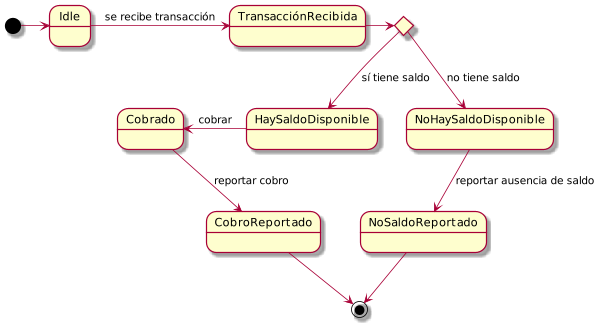
\includegraphics[width=13cm]{./chapters/img/pasarela.png}

    \label{fig:pasarela}
    \caption{Máquina de estados UML para la pasarela de pagos}
\end{figure}

La decisión de si queda saldo o no se realiza de forma aleatoria, con una probabilidad $p = 0.9$ de que quede saldo en la tarjeta y $1- p$ que no quede. En cualquier caso se devuelve un estado del pago: efecutado, o erróneo. Si fue aceptado entonces se procede a guardar toda la información restante en la base de datos y actualizar el estado de la compra de la entrada.
